\section{Dataset Construction}
\label{sec:dataset}

The dataset is the substrate on which every later claim rests, so we describe it in detail. We cover (i) the workload and the instrumentation discipline we applied to it, (ii) the 27 scenario families and how each kind of fault is physically injected into the cluster, (iii) what every label on every window means and how it was created, (iv) how we generated the humanized Jira corpus and what role TAWOS played in that, (v) how the distractor tickets are designed to look identical to real tickets while never matching anything, and (vi) the final numbers --- how many incidents, how many tickets, how many distractors, how many test windows.

\subsection{The workload --- Online Boutique with production-realistic instrumentation}

The workload is Google's \textbf{Online Boutique}, a ten-service e-commerce microservices demo. The services are written in six languages to test polyglot tooling: the frontend, checkout-service, product-catalog-service, and shipping-service are in Go; the cart-service is in C\#/.NET; the payment-service and currency-service are in Node.js; the recommendation-service, email-service, and load-generator are in Python; the ad-service is in Java. The services communicate over gRPC, with a Redis instance (\texttt{redis-cart}) backing the cart-service.

We forked the upstream repository and ran five sequential instrumentation phases (which we call M0 through M5) over roughly three weeks. The single hard rule that governed every change was \emph{anything a real production service would not emit must not be added}. Concretely, we rejected any field that named our scenario taxonomy --- no scenario IDs in span attributes, no fault-type labels in log fields, no alert names tied to our incident families. The rationale was simple: if the telemetry our models train on contains direct leaks of the scenario label, the resulting numbers describe a fictional, easier task than the production task we are trying to model. This made debugging harder (we could not just grep for the fault type) but the dataset defensible.

We added three categories of telemetry. \textbf{Logs.} Every service emits one JSON-formatted log line per RPC it processes, carrying a stable \texttt{trace\_id}, the method name, the peer service it was talking to, the latency in milliseconds, the status code, and an error class if applicable. At every dependency boundary --- wherever a service calls Redis, another gRPC service, or an external HTTP API --- the failure path also emits a structured error record capturing the dependency name, the operation, the error class, and the retry attempt count. A small layer of business events (\texttt{cart\_size\_changed}, \texttt{order\_placed}, \texttt{payment\_charged}, \texttt{recommendation\_returned\_n\_items}) provides domain-level signal. None of these fields encode scenario identity. \textbf{Traces.} We brought every service up to OpenTelemetry parity. The single most-impactful change was on the cart-service: adding the StackExchange.Redis auto-instrumentation produced per-Redis-operation spans for free, which lifted the trace error count for cart-Redis active-fault windows by $3.0\times$ and raised the fraction of cart-Redis windows that had any trace error at all from 50\% to 100\%. We also wrap every error-returning handler in \texttt{RecordError} so the failure attaches to the span, add manual child spans on dependency calls with the OpenTelemetry semantic-convention attributes (\texttt{db.system}, \texttt{db.operation}, \texttt{net.peer.name}, \texttt{rpc.grpc.status\_code}), and emit span events for retries, cache hits, cache misses, and fallbacks. We leave the trace sampler at always-on (a known divergence from production, which typically samples at 1\%--10\%); we favored dataset density over sampling realism and document the gap. \textbf{Metrics.} Every service uses an OpenTelemetry Meter that exports to Prometheus. The RED metrics (Rate, Errors, Duration) are emitted per RPC handler. Per outbound dependency we record client-side metrics labeled by peer service and operation. Business events are counted (\texttt{orders\_placed\_total}, \texttt{payments\_total}, \texttt{cart\_operations\_total}) with label values carefully chosen to never mirror our scenario taxonomy. Runtime gauges (Go GC, .NET GC, Python GC, Node heap, process file descriptors) come from each language's default Prometheus client.

The observability stack we run alongside the application: \textbf{Loki} for log aggregation, \textbf{Tempo} for distributed traces, \textbf{Prometheus} for metrics, \textbf{Alertmanager} for alert routing, and \textbf{Grafana Alloy} as the OpenTelemetry collector. The whole stack runs on a 3-node \texttt{kind} (Kubernetes-in-Docker) cluster on a developer workstation (15.3 GiB host memory budget, $\sim$10--13 GiB sustained); the large-scale collection used a Google Cloud \texttt{e2-standard-16} VM.

\subsection{The scenario library --- 27 families and how each is injected}

A scenario is a single fault we know how to inject and want the model to recognize. We organized them into seven categories. Table~\ref{tab:scenarios} groups them; we then describe each injection mechanism in plain language.

\begin{table}[h]
\centering
\caption{The 27 scenario families.}
\label{tab:scenarios}
\small
\begin{tabularx}{\linewidth}{l X}
\toprule
Category & Families \\
\midrule
Hard service outage (8) & payment-outage, checkout-outage, currency-outage, shipping-outage, recommendation-outage, ad-outage, productcatalog-outage, email-outage \\
Dependency degradation (2) & cart-redis, productcatalog-latency \\
Pod restart / churn (5) & checkout-restart, frontend-restart, single-pod-restart-healthy-replication, flapping-pod, post-deploy-churn \\
Capacity / traffic pressure (4) & frontend-traffic-pressure, scheduled-job-spike, resource-saturation, slow-leak-saturation \\
Near-misses (3) & latency-near-miss-partial-recovery, recovered-in-window, third-party-blip \\
System / network (4) & network-latency, network-packet-loss, network-partition, dns-outage \\
Baseline (1) & baseline-normal \\
\bottomrule
\end{tabularx}
\end{table}

Each scenario uses one of four fault-injection primitives, all implemented as PowerShell wrappers around the Kubernetes API. We describe each:

\paragraph{ScaleDeployment --- scaling a workload to zero replicas.} The cleanest way to take a service offline. We send a \texttt{kubectl scale} command with a target replica count of zero, wait for Kubernetes to terminate the pods, hold the empty state for the active-fault window (typically 90--180 seconds), then restore the original replica count and wait for the pods to come back healthy. This primitive backs every hard service-outage family (payment-outage, checkout-outage, etc.) and also \texttt{cart-redis} (we scale \texttt{redis-cart} to zero). The symptom in the telemetry is unambiguous: callers to the missing service see a flood of \texttt{Unavailable} or \texttt{DeadlineExceeded} gRPC errors; downstream business events drop to zero; Kubernetes events emit \texttt{Killing} on the terminating pods.

\paragraph{SetEnv --- patching an environment variable on a running deployment.} Used for behavioral faults that do not require killing the service. Examples: \texttt{productcatalog-latency-major} sets \texttt{EXTRA\_LATENCY=750ms} on the product-catalog-service so that every catalog query is artificially slowed; \texttt{loadgenerator-traffic-spike-nearmiss} bumps the load-generator's request rate by 3$\times$ for a short window. We patch the deployment via \texttt{kubectl set env}, wait for the rollout, observe through the active-fault window, and restore the original value at the end.

\paragraph{RestartPods --- killing pods matching a selector.} Used for pod-churn and rolling-deployment scenarios. \texttt{checkout-restart} performs a \texttt{kubectl rollout restart} on the checkout-service deployment, which triggers a graceful rolling update. \texttt{single-pod-restart-healthy-replication} kills one pod out of three replicas to test whether the model can tell the difference between an actual outage and a healthy restart. \texttt{flapping-pod} kills the same pod three times within the active-fault window to create a recognizable flap signature. \texttt{dns-outage} reaches into the \texttt{kube-system} namespace and kills the CoreDNS pods, briefly taking down cluster DNS.

\paragraph{RecordOnly --- passive observation, no fault injected.} Used by the \texttt{baseline-normal} family. The cluster runs normally with the load-generator producing realistic traffic; we record the telemetry as a negative example. Baseline windows are essential: a model that has only ever seen incidents will fire on everything.

A fifth class of injection uses the Chaos Mesh operator for network-level faults: \texttt{network-latency} (Chaos Mesh \texttt{NetworkChaos} with a 500ms delay between specified service pairs), \texttt{network-packet-loss} (30\% packet drop), \texttt{network-partition} (full network isolation between two service tiers).

A single \textbf{dataset run} is a sequence of scenarios executed against a freshly deployed cluster. Each scenario contributes one \textbf{incident episode} with three (sometimes four) \textbf{telemetry windows} attached: a \texttt{pre\_fault\_baseline} window (60--120 seconds of normal traffic before the injection), an \texttt{active\_fault} window (the injection itself, 90--180 seconds), and a \texttt{recovery\_window} (90--120 seconds after the fault is cleared). Some scenarios also have an \texttt{observation\_window} for slower-moving conditions like leaks.

\subsection{Per-window labels --- what they mean, how they are created, why they exist}

Every telemetry window carries five categories of labels. This is the language all downstream model training and evaluation speaks, so it is worth defining each label precisely.

\paragraph{(1) Window type --- when in the incident timeline the window lives.}

\begin{itemize}
\item \texttt{pre\_fault\_baseline} --- before the fault was injected. Captures the cluster's normal behavior just before the incident, used as a reference for delta-from-baseline features.
\item \texttt{active\_fault} --- the fault is currently being injected. This is when the symptoms peak.
\item \texttt{recovery\_window} --- the fault has been cleared but residual effects (queue drains, retries, slow client backoffs) may still be visible.
\item \texttt{observation\_window} --- a long passive window for slow-moving faults like memory leaks, where the symptom develops over many minutes.
\end{itemize}

The window-type label comes directly from the orchestration script that ran the scenario, so it is always exact. Window type matters because the same telemetry pattern can mean different things at different points in the timeline: a low-error active-fault window is suspicious (an attack hiding behind quiet metrics?) while a low-error recovery window is normal.

\paragraph{(2) Triage label --- would a senior engineer file a ticket?}

This is the primary label the triage models are trained to predict. Three classes:

\begin{itemize}
\item \texttt{ticket\_worthy} --- a senior on-call engineer would file a Jira ticket if they saw this window. Examples: payment-service outage during checkout, Redis cart degradation, a customer-visible latency regression, a bad config causing failures.
\item \texttt{borderline} --- reasonable engineers would disagree. The fault recovered before significant user impact, or the impact was small enough that filing is a judgment call. Examples: a single-pod restart in a healthy replication group, a brief latency spike that self-recovered, partial degradation under low traffic.
\item \texttt{noise} --- a senior engineer would not file a ticket. Includes normal behavior and recognizable near-misses. Examples: baseline normal traffic, post-deploy churn that settled, high traffic without user impact, a transient third-party blip.
\end{itemize}

We use three classes instead of two on purpose. A binary task forces every edge case into the wrong bucket. The \texttt{borderline} class lets us measure how the model handles genuinely ambiguous windows without penalizing it for refusing to commit. The headline reporting (the ``strict PR-AUC'' number) counts only \texttt{ticket\_worthy} as positive; an ``inclusive PR-AUC'' variant counts \texttt{borderline} as positive too and is reported alongside.

\paragraph{How the triage label is created.} Each scenario YAML carries a \texttt{triage:} block that declares the expected per-window label for each window type. For \texttt{paymentservice-unavailable-critical}, the block reads: pre-fault baseline $\rightarrow$ noise; active fault $\rightarrow$ ticket-worthy (severity critical, components \texttt{[paymentservice, checkoutservice]}, reason class \texttt{dependency\_failure}); recovery $\rightarrow$ borderline. The label source is recorded as \texttt{scenario\_authored} for these. A small subset of windows where the scenario author was uncertain are \texttt{human\_adjudicated} --- a human reviewer looked at the actual collected telemetry and overrode the scenario default. For v3 of the dataset, most labels are \texttt{derived} from existing scenario fields via a deterministic rule; for v4 and later, every borderline and hard-case window is required to be human-adjudicated.

\paragraph{(3) Ticket-side metadata --- severity, components, reason class.}

For windows labeled \texttt{ticket\_worthy}, the dataset also records what the ticket would contain. \texttt{triage\_severity} is one of \texttt{minor / major / critical}, matching the existing Jira-style severity vocabulary. \texttt{triage\_components} is the list of Jira components the ticket would carry (e.g.\ \texttt{[paymentservice, checkoutservice]}); these are the services the ticket would be filed against. \texttt{triage\_reason\_class} is one of seven categories: \texttt{outage}, \texttt{latency\_regression}, \texttt{restart\_with\_impact}, \texttt{bad\_config}, \texttt{capacity}, \texttt{dependency\_failure}, \texttt{data\_consistency}. These three fields are \texttt{null} for borderline and noise windows.

\paragraph{(4) The \texttt{is\_hard\_case} flag.}

A Boolean field marked \texttt{true} when the window is intentionally designed to confuse simple models. Examples of hard cases: a single-pod restart in a 3-replica deployment that should not be ticket-worthy but looks just like a real outage on the symptom side; a near-miss where the fault recovered before user impact, but the active-fault window's telemetry resembles a real incident; a downstream-symptom service (\texttt{checkoutservice}) that surfaces the error but where the root cause is actually a different service (\texttt{paymentservice}). \texttt{is\_hard\_case} is \emph{evaluation-only} --- it is used to stratify metric reporting and to mine training pairs that exercise the model's discrimination, but it is never passed to the model as input.

\paragraph{(5) Memory-match ground truth --- the \texttt{is\_novel} flag and the matched IDs.}

This is the label that makes the dataset memory-augmented rather than just classification. Each window carries:

\begin{itemize}
\item \texttt{matched\_memory\_issue\_ids} --- the list of Jira ticket IDs from the memory corpus that are the ``gold'' matches for retrieval evaluation. Two tickets are matched to a window if they share the same scenario family AND the ticket's \texttt{available\_as\_memory\_from} timestamp is strictly less than the window's start time AND the ticket comes from a different dataset run than the window (to prevent leakage).
\item \texttt{is\_novel} --- a Boolean. \texttt{True} when \texttt{matched\_memory\_issue\_ids} is empty, i.e.\ when no past ticket exists for the window's scenario family. This happens naturally for the first occurrence of a family in chronological order, and synthetically when we use the leave-one-family-out evaluation to hide a family from the corpus.
\end{itemize}

\textbf{What ``novel'' actually means in this dataset.} A novel window is not a window with an unknown bug --- the scenario YAML still knows what fault was injected. It is a window for which the memory corpus, as of the window's timestamp, contains no prior ticket from the same family that the model could plausibly cite. The novelty label is the ground truth for the L3 layer of the cascade and for the novelty-recall headline metric.

\paragraph{(6) Numeric features --- 94 derived columns per window.}

In addition to the labels, every window carries 94 \texttt{triage\_feature\_*} columns pre-computed from the raw telemetry. These are the inputs that the gradient-boosted classifier and the cascade's L1 stacker consume. They split into families: 47 \texttt{delta\_*} columns (active-versus-pre-fault deltas of latency p50/p95, error rate, RPC throughput per status code, business metrics, Kubernetes state), 33 \texttt{m05\_*} columns (absolute current values of RED metrics, business counters, runtime gauges over the most-recent 5-minute window), 6 \texttt{trace\_*} columns (trace count, trace error count, trace error rate, trace latency p50/p95, span count), 3 \texttt{k8s\_*} columns (restart count, warning event count, pod-unavailable count), 3 \texttt{log\_*} columns (log volume counts), and 2 \texttt{metric\_*} columns (container CPU/memory percent, with noted unit caveats). Pre-computing these once is what makes the cascade's inference cost essentially zero.

\paragraph{(7) Free-text evidence --- the \texttt{triage\_evidence\_text} field.}

A human-readable summary of what the window contains, used as the input to text retrievers (BM25, the bi-encoder, the cross-encoder). It interleaves a one-line description of metric anomalies, the top characteristic log lines extracted by an active-vs-baseline diff, and the names of any firing alerts. This text is what stands in for the engineer's view of the window when retrieving past tickets.

\subsection{The humanized Jira memory corpus}

Generating realistic Jira tickets turned out to be harder than generating telemetry. We went through two design iterations.

\paragraph{V1 --- the TIMELINE design (the first attempt).} The first humanizer treated each ticket as a \emph{timeline} of contributions by different personas at different timestamps with different information available at each step. The schema mapped: a \texttt{report} step (the customer-support agent at $t=0$ who has seen only the first 30 seconds), an \texttt{ack} step (the on-call SRE at $t=+3$min who has seen the first three minutes), one or more \texttt{hypothesis} steps (engineers at $t=+5$ to $+10$min who have seen the active-fault window), an optional \texttt{redirect} step (the senior SRE who points out that the first guess was wrong), and a \texttt{resolve} step (the fix-author at $t=+30$min who has seen the whole picture). Nine personas were defined: \texttt{cs-agent}, \texttt{oncall-sre}, \texttt{junior-eng}, \texttt{frontend-eng}, \texttt{backend-eng}, \texttt{senior-sre}, \texttt{eng-mgr}, \texttt{db-team}, \texttt{fix-author}. Each persona has a vocabulary distribution: a senior SRE writes ``redis ctimeout x12 on cart-redis:6379'' in nine words; a junior writes a paragraph; a customer-support forward says ``customers can't add to cart.''

V1 enforced five strict leakage-safety rules. First, the LLM never sees any scenario ID, fault type, or any of the strings \texttt{fault}, \texttt{synthetic}, \texttt{injected}, \texttt{chaos-mesh}, \texttt{lab}, \texttt{nearmiss}, \texttt{scenario}, \texttt{borderline}, etc. A sanitizer asserts these tokens never appear in the LLM input and fails loudly if they do. Second, before generation, the LLM is told the user-visible symptom phrase (``users seeing cart-not-loading after add-to-cart'') rather than the technical fault name (\texttt{cart-redis-degradation-critical}). Third, 10--15\% of tickets deliberately have the wrong initial component attribution --- the first commenters frame it as a \texttt{checkoutservice} problem when the real cause is \texttt{productcatalog-latency}; a senior SRE later redirects. This teaches the model that the ``components'' field is a hint, not an oracle. Fourth, the reporter and early commenters must quote specific log lines and metric values from the actual telemetry rather than summarizing; quotes are paraphrased through persona voice. Fifth, 10--20\% of borderline tickets and 30--40\% of noise tickets close as ``cannot reproduce'', ``self-resolved'', ``not a bug'', or ``duplicate of TICKET-1234'' so the model learns that not every ticket is a real bug.

V1 shipped (347 humanized tickets) but the resulting corpus was off-distribution: the leading text of each ticket was the cs-agent voice (``Customer reports slow site performance...''), which meant BM25 indexed customer-support vocabulary instead of engineer vocabulary. Retrieval lift was only marginal.

\paragraph{V2 --- the TAWOS-grounded engineer-voice redesign.}

The V2 redesign was driven by a direct empirical study of the TAWOS dataset. We loaded TAWOS (458{,}232 real Jira issues from 39 open-source projects, in a local MySQL 8.0 instance) and queried for the distributions on dimensions that matter for the humanizer:

\begin{itemize}
\item \textbf{Description length} --- TAWOS descriptions are \emph{much shorter} than our V1 had assumed: median 200--500 characters; 56\% are under 500 characters; 82\% are under 1{,}000 characters. V1 had been emitting 1.5--3K characters of multi-paragraph markdown.
\item \textbf{Pasted log or stack-trace blocks} --- in TAWOS, 20.5\% of bug tickets carry a separate code-block field (\texttt{Description\_Code}); 16.5\% have substantial code content. Real Jira already has a structural separation between prose and pasted blocks.
\item \textbf{Comments per issue} --- 36\% of tickets have 1 comment; 43\% have 2--5; 14\% have 6--15; 4\% have more than 15.
\item \textbf{Resolution time} --- 4\% close in under an hour, 11\% in 1h--1d, 20\% in 1d--1wk, 25\% in 1wk--1mo, 40\% in more than a month.
\item \textbf{Resolution outcome} --- 60\% Fixed, 15\% Won't Fix, 12\% Duplicate, 4\% Cannot Reproduce, 3\% Not A Bug, 4\% Timed Out.
\item \textbf{Voice} --- terse engineer pager-speak, raw log pastes mid-thread, multi-month gaps between comments, no markdown headers.
\item \textbf{Stack-trace token frequency} --- on tickets with code blocks, Java tokens dominate: \texttt{com.} 38\%, \texttt{Exception} 37\%, \texttt{java.} 33\%, \texttt{org.} 30\%, \texttt{Caused by:} 12\%, \texttt{NullPointerException} 7\%.
\end{itemize}

The structurally most-surprising find was the TAWOS column split: real Jira already separates prose (\texttt{Description\_Text}, \texttt{Comment\_Text}) from pasted blocks (\texttt{Description\_Code}, \texttt{Comment\_Code}). V1 had collapsed these into a single field and forced the LLM to weave logs into narrative --- exactly the channel where leakage and voice pollution sneak in.

V2 inherits this split. Every humanized ticket now has:

\begin{itemize}
\item \texttt{description} --- prose only, 200--500 characters, no markdown headers, engineer pager-speak.
\item \texttt{description\_code} --- 1--5 pasted log lines drawn from a \emph{characteristic-log-line extractor} that runs an active-versus-baseline diff over Loki data and surfaces lines that are rare in baseline but present in the fault window. \textbf{Target coverage $\geq 80\%$; final V2 corpus achieved 90.2\%.}
\item \texttt{comments} --- variable count sampled from the empirical TAWOS distribution, each with a \texttt{body} (prose) and an optional \texttt{body\_code} (pasted block).
\item \texttt{resolution} --- one of the seven TAWOS-empirical outcomes.
\item \texttt{resolution\_time\_s} --- sampled from the empirical TAWOS distribution.
\end{itemize}

\paragraph{Evidence at generation time.} The V2 humanizer reads a multi-channel \texttt{EvidenceBundle} for each ticket: the log signature (1--5 characteristic lines), paraphrased metric observations (``trace p95 latency +6.35s vs baseline'', ``RPC OK throughput $-38.5$/sec'', ``+9 pod restarts vs baseline''), a trace summary, the Kubernetes state (restart count, warning event count), the names of the firing alerts (``CartServiceP99LatencyHigh''), and a symptom phrase from the leakage-safe symptom map. Different personas get different slices of this bundle: the customer-support agent sees only the symptom phrase; the on-call SRE sees the alert names and the high-level trace summary; the senior SRE sees the full bundle.

\paragraph{Coverage rule --- one ticket per injected fault.} Unlike TAWOS where coverage is sparse, our data scale is fundamentally bounded (one project, five days of raw collection), so we cannot afford to skip any injected fault. The build-time check asserts that every injection ID has exactly one corresponding humanized ticket. For \texttt{critical} severity faults we allow 1--3 tickets per injection (the bug ticket always; optionally a follow-up reliability ticket written 1--3 days later; optionally a postmortem ticket written 1--2 weeks later that cross-links to the original). For \texttt{major} severity, 1--2 tickets; for \texttt{minor}, 1 ticket strictly. Follow-up tickets carry an \texttt{is\_followup\_of} pointer to the parent.

\paragraph{Reproducibility.} Every humanized ticket gets a manifest entry capturing the episode it was generated for, the persona seeds used, the SHA-256 hash of every prompt that hit the LLM, the LM Studio model ID and temperature, the sanitizer version, the symptom-map version, and the git SHA of the generator. The LLM is Qwen 3.6 35B-A3B (a 35-billion-parameter Mixture-of-Experts model with 3 billion active parameters per token) served locally via LM Studio with MoE offload to system RAM. At temperature 0.7 the model produces $\sim$10\% lexical variance across reruns, well below the bootstrap confidence-interval widths in our metrics.

\subsection{Distractor tickets --- the same shape, but unrelated}

Coverage alone tells us only that \emph{some} ticket exists for each fault; it does not tell us whether the model retrieves the \emph{right} ticket. To test retrieval precision under realistic noise we mix in 110 \textbf{distractor tickets}: well-formed Jira issues that describe plausible incidents that never happened in our corpus. The distractor pool was minted under three sourcing strategies:

\begin{itemize}
\item \textbf{TAWOS-sampled (60 tickets, 55\% of the pool).} Real bug reports pulled directly from the TAWOS MySQL database, filtered to projects most similar to ours in style (MongoDB SERVER, Mesos, Mule, Hyperledger Fabric). Project-specific nouns (server names, branch names, internal URLs) are scrubbed; the original real-engineer voice is preserved. These are the ``gold standard'' distractors precisely because their voice is real engineer voice that no synthetic generator can quite match. They do not go through our persona system at all.
\item \textbf{In-architecture-but-never-happened (25 tickets).} Synthetic incidents in services we have, but for fault modes we never injected (e.g.\ ``payment service rate limiter dropping calls'' when we never injected that fault). These are the hardest distractors: they share service-name lexical overlap with real tickets, so they test whether the model is matching on actual log evidence or just on shared vocabulary.
\item \textbf{Cross-architecture (25 tickets).} Synthetic incidents in components we do not have (Kafka consumer lag, Spark job OOM, Postgres replication lag). High retrieval-confusion potential because the infrastructure vocabulary is engineer-realistic and overlaps with generic incident text.
\end{itemize}

To prevent voice from becoming a tell, the cross-architecture and in-architecture-never-happened distractors use the same nine personas as the real V2 tickets, but the avatar names are drawn from a wider pool so the same Sarah Chen does not handle both a real cart-redis incident and a fake Kafka distractor. The TAWOS-sampled distractors are kept verbatim, with only the project-noun scrub applied. Distractor resolution times are clipped to $[1\text{h}, 5\text{d}]$ to match our 5-day collection horizon so that a model correlating ``resolution time $>$ 1 week'' with ``is distractor'' would not get a free shortcut.

Each distractor carries a Boolean \texttt{is\_distractor} field in the schema, but \textbf{this field is never visible to the model at retrieval time}. It is evaluation-only metadata. The G6 robustness sweep (Section~\ref{sec:experiments}) mixes distractors into memory at ratios of $\{0, 10, 25, 50\}\%$ and measures how Hit@K degrades.

\subsection{Run orchestration and the data layout in plain language}

A dataset run goes through three layers of persistence so that any number we report can be regenerated.

\textbf{Layer 1 --- raw evidence.} Each run produces, per window, the Loki log records that fell in that time range, the Tempo trace JSON files, the Prometheus metric query results, the Kubernetes events, the alerts that fired (as named alerts, not metric expressions), and the shadow Jira issues created for episodes the scenario marked as ticket-worthy. The shadow Jira record carries 10 top-level keys including metadata (summary, components, severity, labels), telemetry links (the IDs of the windows that triggered it, the alert fingerprints, the trace IDs), and a synthetic activity timeline (status changes, comments, watchers).

\textbf{Layer 2 --- per-run derived.} A build step turns the raw evidence into model-ready files. Each window becomes a row in a triage examples file containing the labels (window type, triage class, severity, components, reason class, is-hard-case), the matched memory issue IDs, the novelty flag, and the 94 derived numeric features. A separate window-memory-matchings file records the ground-truth links from windows to past tickets. A windows file holds the evidence summaries the text retrievers consume. An issues file holds this run's contribution to the global Jira corpus.

\textbf{Layer 3 --- global derived.} An aggregation step combines all runs into a global view: a global triage examples file with all windows across all runs, the time-ordered Jira memory corpus with each ticket's \texttt{available\_as\_memory\_from} timestamp, the train / validation / test split manifest (and a separate leave-one-family-out manifest), and the schema descriptors.

A validation step at the end enforces that every record carries the dataset run ID, every episode has at least one window, every Jira shadow issue links to an episode and at least one window, every window has at least one raw export, negative windows are present, severities are in $\{none, minor, major, critical\}$, and time ranges are non-overlapping where expected.

\subsection{Final dataset statistics}

Table~\ref{tab:dataset-numbers} consolidates the numbers a reader is most likely to ask about.

\begin{table}[h]
\centering
\caption{Locked dataset statistics. Global dataset ID: \texttt{2026-05-25-dataset-v5-large-global}.}
\label{tab:dataset-numbers}
\small
\begin{tabular}{lr}
\toprule
Item & Count \\
\midrule
Dataset runs (independent fault-injection experiments) & 100 \\
Scenario families & 27 \\
Total incident episodes injected (with shadow Jira) & $\sim$ 720 \\
Total telemetry windows produced & 6{,}720 \\
v2 in-distribution split --- train & 4{,}701 \\
v2 in-distribution split --- validation & 1{,}011 \\
v2 in-distribution split --- test & 1{,}008 \\
\quad Test windows with at least one gold-match past ticket & 331 \\
\quad Test windows truly novel (no past match exists) & 677 \\
Humanized V2 Jira memory corpus (real tickets) & 347 \\
\quad Tickets with at least one \texttt{description\_code} block & 313 (90.2\%) \\
\quad Coverage: real tickets per injected fault & 1.0 (exact, build-asserted) \\
Distractor pool & 110 \\
\quad TAWOS-sampled & 60 (55\%) \\
\quad In-architecture-never-happened & 25 (23\%) \\
\quad Cross-architecture & 25 (23\%) \\
Combined memory + distractor corpus & 457 tickets \\
Derived numeric features per window & 94 \\
Raw evidence size (logs + traces + metrics + k8s) & $\sim$ 10 GB compressed \\
\bottomrule
\end{tabular}
\end{table}

The split is chronological and family-stratified: every one of the 27 scenario families appears in train, validation, and test, but with disjoint fault-injection runs in each split. This is the ``in-distribution'' regime, which is what a mature SRE team would see after a few months of operation. A complementary leave-one-family-out evaluation (Section~\ref{sec:experiments}) tests the harder ``orphan family'' regime.

Figure~\ref{fig:anchor-depth} shows the depth-stratified retrieval curve --- how Hit@5 climbs as the memory corpus accumulates more past tickets sharing the test window's family. This was the original headline finding from the project's Phase A and remains true through every subsequent generation.

\begin{figure}[h]
\centering
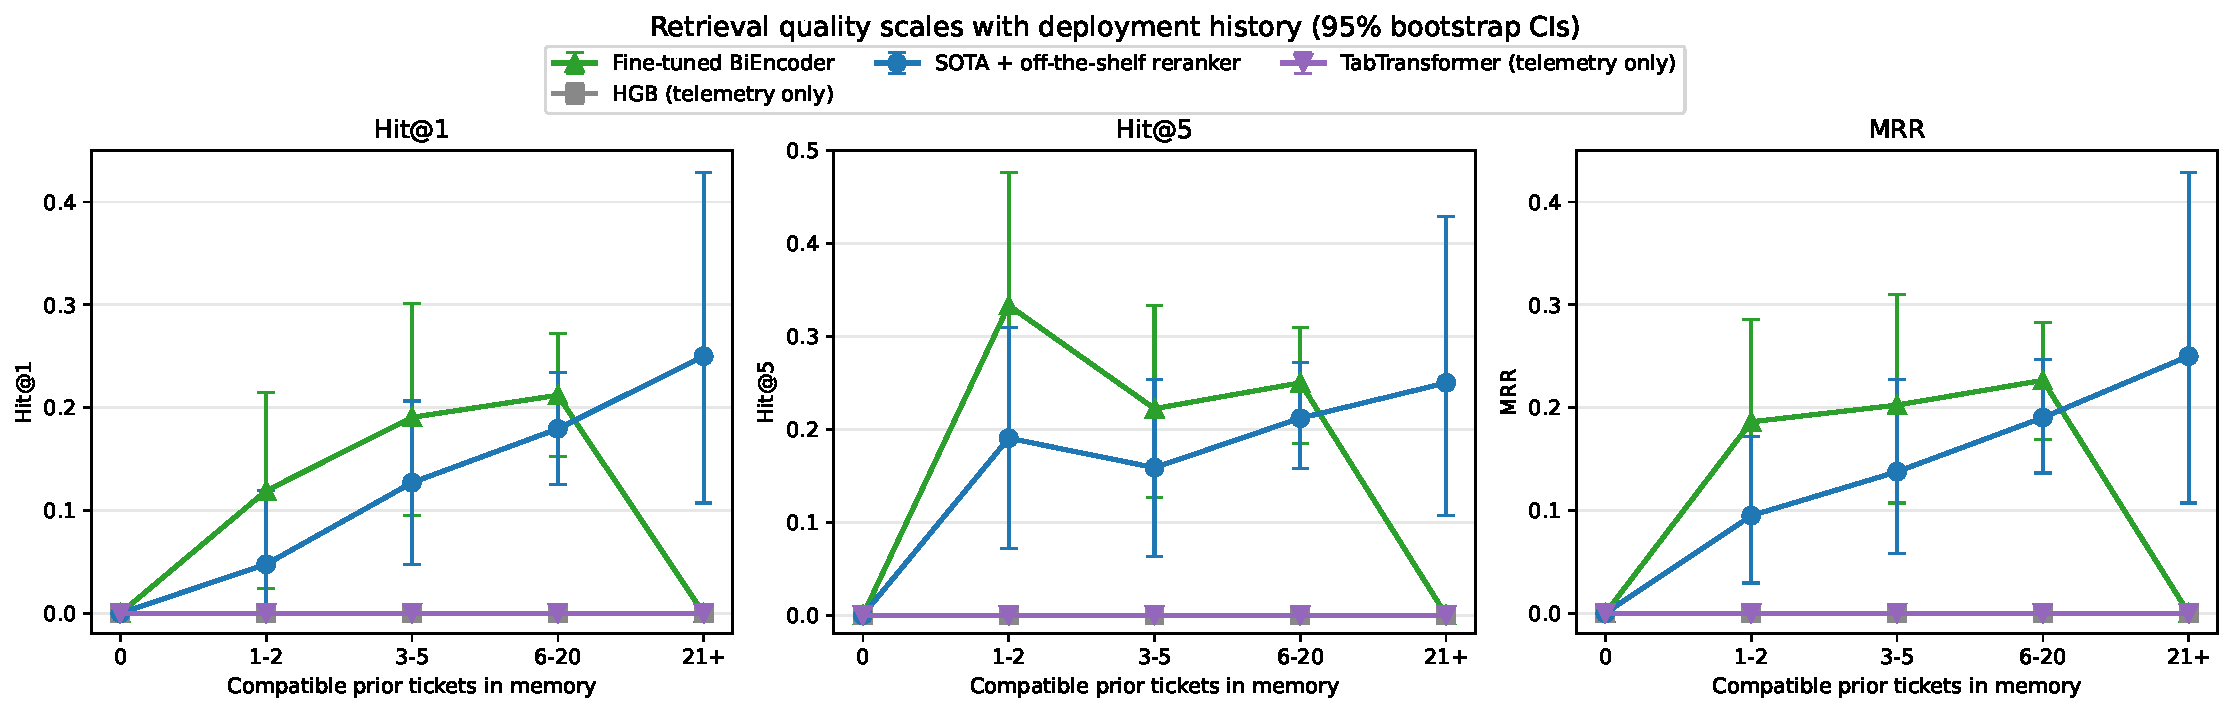
\includegraphics[width=0.85\linewidth]{figures/anchor_combined.pdf}
\caption{Depth-stratified retrieval: Hit@5 versus the number of prior memory tickets sharing the test window's scenario family. Retrieval quality scales with deployment history --- the operational property that motivates memory-augmented triage.}
\label{fig:anchor-depth}
\end{figure}
